\documentclass{beamer}

\usepackage[utf8x]{inputenc}
\usepackage{graphicx}
\usepackage{setspace}
\usepackage{tikz}
\usepackage{algorithm}
\usepackage{algpseudocode}
\usepackage{array}
\usepackage{amsmath}
\usepackage{pgfpages}

\usetikzlibrary{arrows,decorations.pathmorphing,backgrounds,positioning,fit,petri}

\usetheme{PaloAlto}
\usecolortheme{seahorse}
\usefonttheme{structurebold}

\setbeamertemplate{footline}
{
}
%\setbeameroption{show notes on second screen}

\title{Docker for Fun and Profit}
\author{Luka Stojanović}
\institute{
  luka@magrathea.rs \\
  Seven Bridges Genomics
}
\date{Startit Tech Meetup \#3\\ 05. 12. 2013.}
\subject{Software engineering}

\begin{document}
  \begin{frame}
    \titlepage
  \end{frame}
  
  \begin{frame}
    \frametitle{Outline}
    \tableofcontents
  \end{frame}
  
  \section{What is Docker?}
  \begin{frame}
    \frametitle{What is Docker?}
    %\begin{block}{Title}
    %    Text
    %\end{block}
    \begin{block}{\url{http://www.docker.io}}
    	Docker is an open-source project to easily create lightweight, 
    	portable, self-sufficient containers from any application
    \end{block}

    \centering
	    
\includegraphics[scale=0.5]{homepage-docker-logo.png}
    \note{
		Now, questions
  	}
    
    %\begin{itemize}
    %    \item Item
    %\end{itemize}
    
  \end{frame}
  
  \begin{frame}
  	\frametitle{What does it mean?}
	\begin{itemize}  	
  		\item Open source
  	
	    \begin{itemize}
    		\item Code available on Github: \url{https://github.com/dotcloud/docker}
        	\item Written in Go
	        \item Actively developed, lots of community contributors
	    \end{itemize}
    
    \item Lightweight, portable, self-sufficient containers
    	\begin{itemize}
    		\item No virtual machine, runs on host hardware/kernel
			\item Isolated from host using kernel features such as control groups,
				process/network namespacing
	    \end{itemize}
    
    \item ...from any application
    	\begin{itemize}
    		\item Point of view that influences design
	    \end{itemize}
    \note{
		Code not of a supreme quality, but improving \\
		Go is easy to read and understand \\
		LXC is virtual-machine oriented \\
  	}
    \end{itemize}
    
  \end{frame}
  
  \begin{frame}
  	\frametitle{Origin}
  	\begin{itemize}
		\item Created by than Dotcloud to support their PaaS business
  		\item Open-sourced as 'cool peace of tech'
  		\item Caught like wildfire - company renamed recently to Docker inc.
  	\end{itemize}
  \end{frame}
  
  \begin{frame}
    \frametitle{What does it do?}
    \begin{itemize}
    	\item System daemon with an HTTP API
        \item Command line tool
        \item Image packaging format
	    \item Repository with pre-cooked images
	\end{itemize}
	\note{Show some cli usage, process on host\\
	This is where they screwed up a bit}
  \end{frame}
  
  \begin{frame}
  	\frametitle{But I heard it's picky about Linux version}
	\begin{itemize}
		\item It was, but not that much
  		\item As of last week and version 0.7 it's even less picky
  		\item Plans to make it cross platform (Linux/BSD/Solaris)
  	\end{itemize}
  \end{frame}
  
  \section{What's Inside the Box?}
  \begin{frame}
  	\frametitle{What's Inside the Box?}
    \begin{itemize}
    	\item Linux containers (lxc)
        \item Control groups (cgroups)
        \item Union mount file system (aufs)
    \end{itemize}
    \note{
		It's important to know what's inside the box.\\
		Maybe Docker doesn't quite suit you, or it does, but you want to tweak things a bit\\
		Or maybe you'll find those technologies useful beside docker
  	}
  \end{frame}
    
  \section{sbgsdk}
  \begin{frame}
    \frametitle{Seven Bridges}
    \centering
	    
\includegraphics[scale=1]{sbg-logo.eps}
    \begin{itemize}
    	\item Boston/Belgrade based BioIT startup
    	\item We're hiring! Checkout \url{https://jobs.sbgenomics.com}
    	\item Platform for processing genome data, data management, visualization, project coordination
    	\item Lots of 3rd party apps
    	\item One app does only part of the job - pipelines
    \end{itemize}
    \note{
		jobs: platform engineer, pipeline engineer, front-end developer\\
		show pipeline    
    }
  \end{frame}

  \begin{frame}
    \frametitle{Use case}
    \begin{itemize}
    	\item We want to enable outside developers to deploy applications to our platform
    	\item Reproducibility is a big concern
    	\item Process isolation, resource control - Yes, please
    \end{itemize}
    \note{
		two use cases, researcher and corp \\
		science, bitches \\
		
    }
  \end{frame}
  
  \begin{frame}
  	\frametitle{SDK}
  	\begin{itemize}
    	\item Application protocol
    	\item Python implementation
    	\item Docker as a package format: existing tooling, only diff is transported
    	\item Docker as a system service: daemon runs and monitors processes, process isolation, resource control
    \end{itemize}
    
    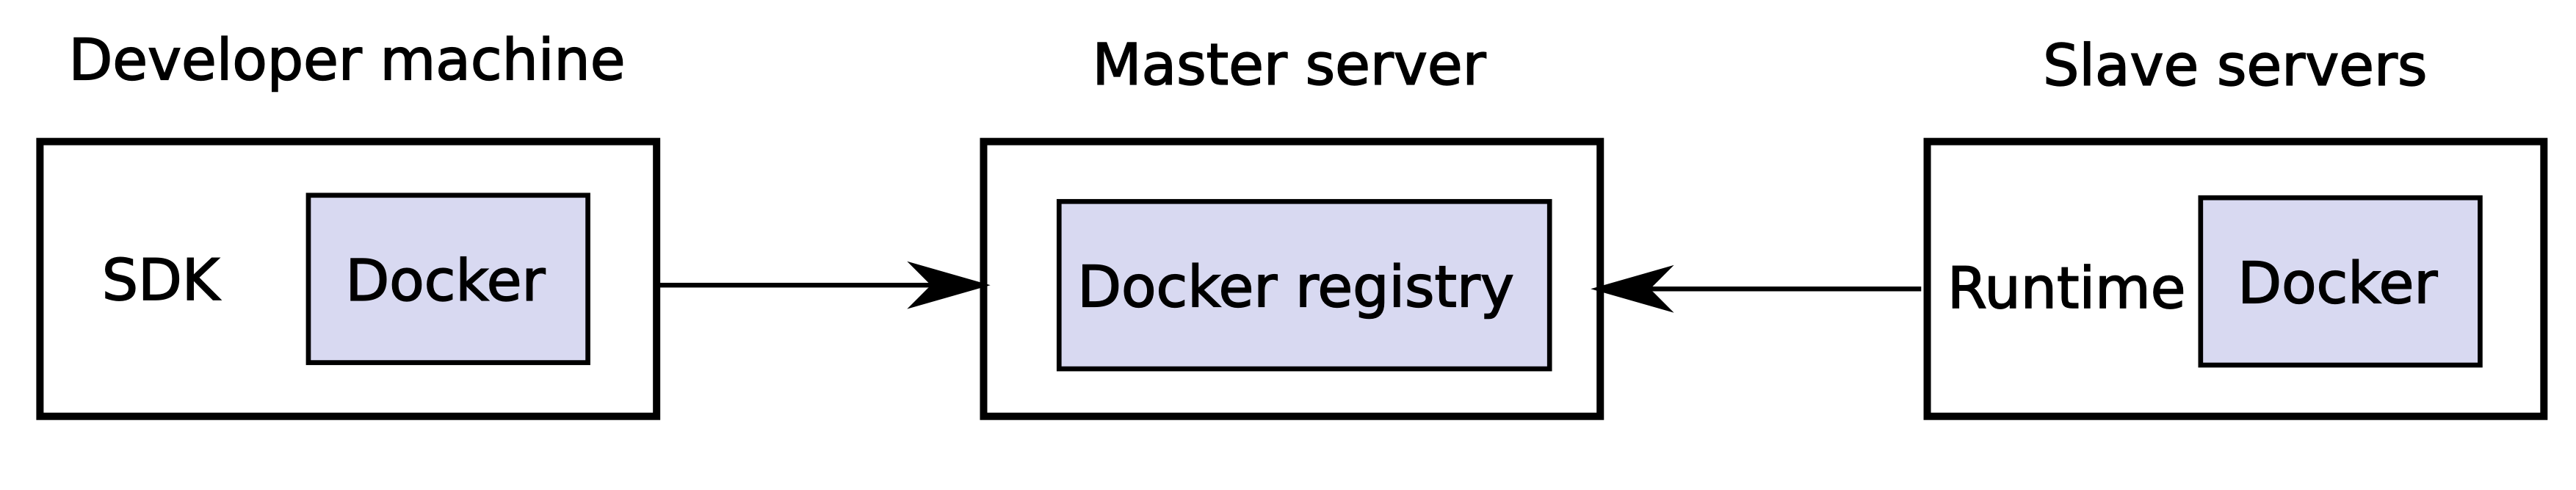
\includegraphics[scale=0.33]{arch.png}
    \note{
     think CGI\\
     
    }
  \end{frame}

  
\end{document}